\chapter{Реализация норадреналиновой системы}
\label{chap:nora}
Норадреналиновая система являлась последним недостающим элементом когнитивной архитектуры NeuCogAr, при уже реализованных дофаминовой и серотониновой системах. В этой главе описываются базовые принципы динамики концентрации норадреналина, их программная реализация и тестирование.


Нейромедиатор норадреналин (он же норэпинефрин) относится к биогенным аминам, группе катехоламинов, он активно используется симпатической периферийной нервной системой (мобилизует организм к действию) и центральной нервной системой (мобилизует мозг для действий). Норадренергические нейроны в мозге немногочисленны: около 4000 в основном месте залегания — голубоватом пятне (locus coeruleus), около 3000 в ядрах солитарного тракта (nucleus tractus solitarii). Но эти нейроны посылают проекции во многие области мозга и оказывают на них значительное влияние. Активность норадренергических нейронов связана с разнообразными реакциями: на стресс, на неожиданность, на такие раздражители как боль, жар или холод, затруднение дыхания. Во время сна активность в очаге голубоватого пятна падает, во время бодрствования работает на уровне минимально необходимом, резко повышается при появлении стимула, привлекающего внимание. Высокий уровень деятельности норадреналина вызывает повышение бдительности и скорости реакции, фокусировку внимания, улучшение обработки сенсорных входов, повышение уровня возбуждения.


Контроль над такими когнитивными процессами как внимание, возбуждение и бдительность необходим для реализации эмоциональных состояний злости, удивления, страдания и заинтересованности. Поэтому, по аналогии с существующими моделями дофамина и серотонина, принципы работы норадреналина были реализованы в виде нового модуля, добавленного в NEST Simulator.


Модель механизма изменения концентрации норадреналина основана на модели, предложенной Е. Ижикевичем для описания динамики концентрации дофамина после серии событий (поощрений). В работе Е. Ижикевича принципы всплеска дофамина в ответ на поощрение иллюстрируются собаками Павлова, вырабатывавшими рефлексы в связи с тем, какие действия сопровождались наградой. Исследуя механизм вырабатываемого рефлекса, неясно, как мозг «запоминает» цепочки нейронов, активность которых вознаграждалась - ведь между событием и наградой проходило несколько секунд (слишком долго для стандартного алгоритма спайковой пластичности).


Е. Ижикевич вводит понятие «сигнализирующей отметки» (eligibility trace) — своеобразных следов, оставляемых в синапсе после того, как по нему проходит спайк. В реальном биологическом мозге это какие-либо кислоты, активизируемые ненадолго, но дольше, чем на пару секунд. Затем, как проиллюстрировано на рис. 3, награда (поощрение) вызывает резкое повышение уровня дофамина, и тогда, благодаря совпадению всплеска дофамина с «сигнализирующей отметкой» в синапсе, синаптическая связь усиливается (а в модели увеличивается её «вес»).


\begin{figure}
	\centering
	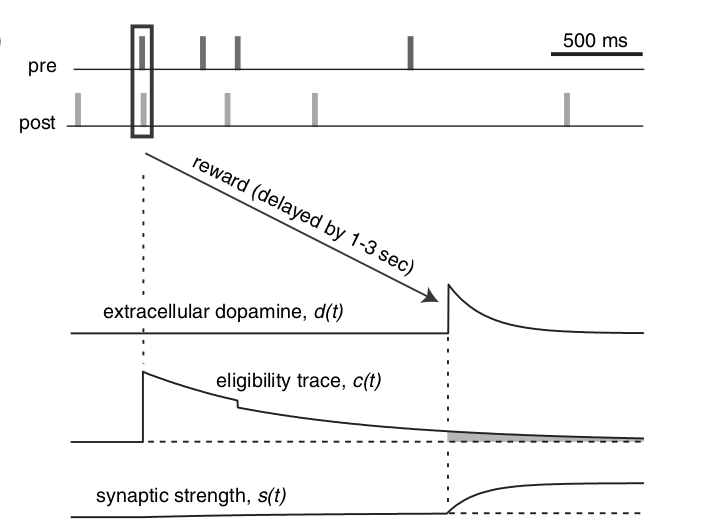
\includegraphics[width=\linewidth]{izhikevich}
	\caption{Иллюстрация процесса усиления синаптической связи из работы \cite{izh}. Происходит благодаря повышению уровня дофамина и имеюшейся у синапса «сигнальной отметки» (eligibility trace), которая возникла секундами раньше.}
	\label{fig:sample_figure}
\end{figure}


Cохранено предположение, что в синапсах, соединяющих два возбуждающих нейрона, действует спайковая пластичность, зависящая от времени. Модель Е. Ижикевича для дофамина была представлена в виде набора определяющих уравнений. Опираясь на них, для сети нейронов, где 80\% возбуждающие и 20\% ингибирующие, для норадреналина составлены следующие уравнения:


1) Зависимость потенциала мембраны v от переменной восстановления мембраны u. The dynamics of each neuron is such that the membrane potential $v$ of each neuron at each moment (new current potential $\dot{v}$) depends on abstract membrane recovery variable $u$ (new current value $\dot{u}$) \cite{tactile}:

\begin{equation} \label{eq:1}
\dot{v} = k (v - v_{rest})(v - v_{thresh}) - u + I
\end{equation}


\begin{equation} \label{eq:2}
%SD
% u =  a*b*(v - v_{rest}) - u 
\dot{u}=  a*b*(v - v_{rest}) - u
\end{equation}


\begin{equation}\label{eq:3}
if (v >= 30 [mV]) : \{v = - 65 [mV], u = u + 2 [mV]\}
\end{equation}


In our model, membrane voltage threshold $v_{thresh}$ and resting potential $v_{rest}$ are constant, and the synaptic current input $I$ (the current flowing in a neuron) has an exponential shape.
The spike occurs when the membrane potential is higher than -50 mV, and then the membrane potential recovers: $v$ decreases to -65 mV, $u$ increases by 2 mV. 
We set $a$ to 0.02, $b$ to 0.2, $k$ to 1. 

Following Izhikevich, the STDP model \cite{stdp} does not change the synaptic weights directly, but instead it modulates weights through a temporal eligibility trace (as it will be shown in \ref{eq:6}. 
The variation of the eligibility trace \textit{c} (new current eligibility trace $\dot{c}$) is described as follows: 


\begin{equation}\label{eq:4}
\dot{c} =  -\frac{c}{\tau_c} + A^+e^{\frac{(t_{pre} - t_{post})}{\tau^+}}\delta(t - t_{post})  -A^-e^{  \frac{(t_{pre} - t_{post})}{\tau^-}}\delta(t - t_{pre} )
\end{equation}


where $t_{pre}$ and $t_{post}$ are the times of a pre- or post-synaptic spike, $A^+$ and $A^-$ are the amplitudes of the weight change, $\tau_+$ and $\tau_-$ are constant rates, $\delta(t)$ is  the Dirac delta function that step-increases the variable $c$. 
The eligibility trace decays at the rate of $\tau_c$. 


The concentration of noradrenaline also impacts the modulation of synaptic weights \cite{nora1}\cite{nora2}, as shown in (6).

The noradrenaline concentration $n$ decreases exponentially with time (natural fade rate is $\tau_n$), and increases depending on salient, novel events: 


\begin{equation}\label{eq:5}
\dot{n} = -\frac{n}{\tau_n} + p_{nov}n (\delta(t - t_n)p_{rew} + \delta(t - t_n)p_{pun})
\end{equation}


where $p_{punish}$ is a punishment (stressor) event, $p_{rew}$ is a reward event, $p_{nov}$ is the probability of the event being novel and unexpected (salient). 
The noradrenaline concentration cannot go below zero: it increases with stressors, if $p_{nov}$ is bigger than zero (a sudden stress), as well as with rewards, if $p_{rew}$ is bigger than zero (a surprise reward). 

The excitatory synaptic weight $w$ (new current value $\dot{w}$) is not changed directly in the model. Instead, it is modulated proportionally to relative concentration of noradrenaline $n$ (to its baseline level $b_n$), multiplied by eligibility trace $c$: 

\begin{equation}\label{eq:6}
\dot{w} = c(n - b_n)
\end{equation}

Модель была протестирована на языке MATLAB, вместе с уже реализованными моделями серотонина и дофамина, в следующих условиях:
\begin{itemize}
\item Задана сеть из 1000 нейронов с синаптической пластичностью, зависящей от времени;
\item 100 синапсов на нейрон;
\item Задержка проводимости 1 мс;
\item Максимальный вес синапса 5;
\item Потенциал покоя мембраны -65 mV;
\end{itemize}

\begin{figure}
	\centering
	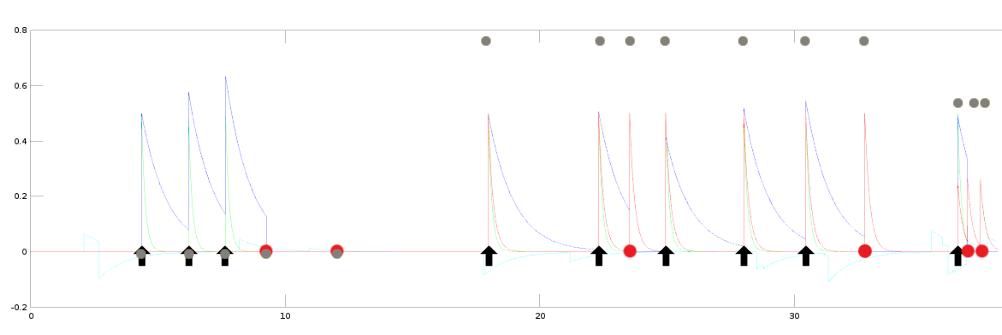
\includegraphics[width=\linewidth]{BIG_matlab_NA_with_NOV}
	\caption{Изменение концентрации норадреналина (красный), дофамина (зелёный) и серотонина (синий) в зависимости от примененных к ним стимулов: поощрение (чёрная стрелка), стресс (красный кружок), новизна (серый кружок).}
	\label{fig:sample_figure}
\end{figure}

На рис. 8 изображён результат работы нейронной сети из 1000 нейронов в течение 500 миллисекунд, на которую подавались случайным образом события поощрения и стресса. Каждое из событий имело уровень неожиданности нулевой (полностью предсказуемое событие, первая треть временной шкалы), средний (последняя треть временной шкалы) или высокий (резкое, внезапное событие).
При абсолютной предсказуемости событий концентрация норадреналина не поднимается совсем, тогда как уровни серотонина и дофамина одинаково поднимаются от предсказуемой награды, от предсказуемого наказания (стресса) уровень серотонина обрушивается вниз, а дофамин на наказание не реагирует.
При событии резком, сколько-нибудь внезапном, будь то поощрение или наказание, концентрация норадреналина повышается; реакция серотонина и дофамина на эти события остаётся той же, что и когда они были «ожидаемы», «предсказаны» системой.


Полученные реакции соответствуют экспериментальным результатам исследовательских работ разных лет [9. Viljoen M., Panzer A.  The central noradrenergic system: an overview. African Journal of Psychiatry vol.10:135-141. (2007)  doi:10.4314/ajpsy.v10i3.30245
10. Delaney A.J., Crane J.W., Sah P. Noradrenaline Modulates Transmission at a
Central Synapse by a Presynaptic Mechanism. Neuron vol. 56: 880–892. (2007)  doi:10.1016/j.neuron.2007.10.022
11. S.J. Grant, D.E. Redmond Jr., Neuronal activity of the locus ceruleus in awake Macaca arctoides, Exp. Neurol. 84 (1984) 701–708.
12. A.M. Thierry, F. Javoy, J. Glowinski, S.S. Kety, Effects of stress on the metabolism of norepinephrine, dopamine and serotonin in the central nervous system of the rat. I. Modifications of norepinephrine turnover, J. Pharmacol. Exp. Ther. 163 (1968) 163–171.]. Поскольку результат, показанный моделью норадреналина в MATLAB, был убедителен, то модель была перенесена на язык c++ и добавлена в инструмент симулирования нейронных спайковых сетей NEST-2.12.0 в качестве нового модуля. Работа модуля была протестирована на простой модели из трёх нейронов: пресинаптический нейрон, постсинаптический нейрон и норадренергический нейрон. Модель симулировала процесс нейромодуляции, усиливающий связь между обычными нейронами в случае, если между ними произошёл спайк при высокой концентрации нейромедиатора норадреналин. Для этого к каждому из трёх нейронов были подключены генераторы спайков в 250 Гц и детекторы спайков. Модель была запущена дважды: с активацией норадреналина и без. Симуляции длились по 3000 миллисекунд.


\begin{figure}
	\centering
	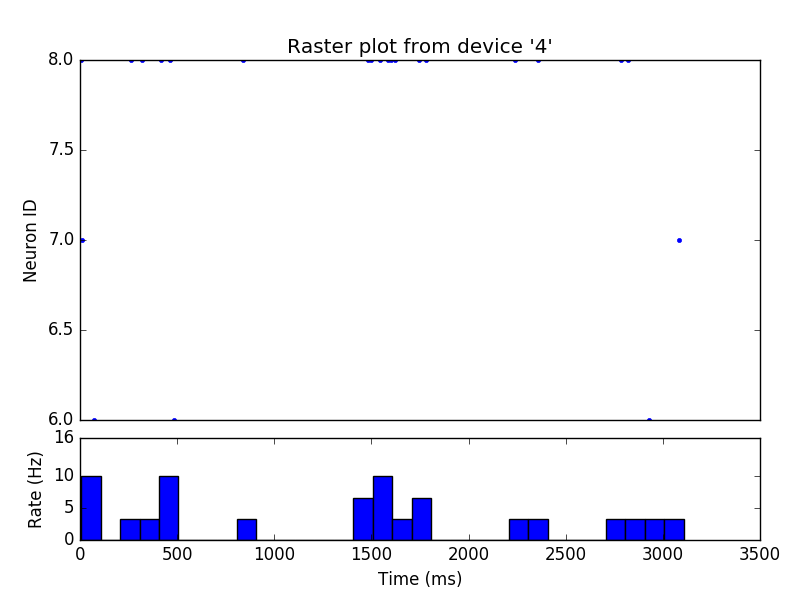
\includegraphics[width=\linewidth]{spikes_250}
	\caption{Спайковая активность на нейроне 6 (пресинаптический), нейроне 7 (постсинаптический), нейроне 8 (норадренергический).}
	\label{fig:spikes_250}
\end{figure}


\begin{figure}
	\centering
	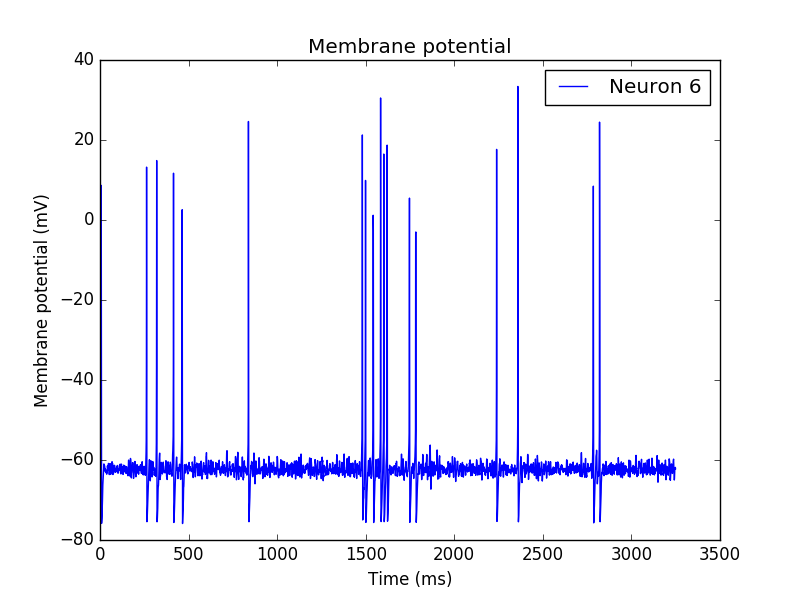
\includegraphics[width=\linewidth]{voltage_250}
	\caption{Динамика концентрации норадреналина.}
	\label{fig:voltage_250}
\end{figure}


На рисунке ~\ref{fig:spikes_250} показана спайковая активность каждого из трёх нейронов в эксперименте с активированным норадреналином. На рисунке ~\ref{fig:voltage_250} — изменение концентрации норадреналина со временем. Сильное увеличение концентрации наступает после относительно «длительного» отсутствия спайков, поскольку после «тишины» в 400 миллисекунд новый спайк имеет уже ненулевой фактор внезапности, считается неожиданным. В случае же спайков идущих подряд концентрация падает. То, как сочетание спайков и изменений концентрации повлияло на силу связи (вес синапса) между пресинаптическим и постсинаптическим нейронами, показывает рисунок ~\ref{fig:w_dynamic_250_with_nora}. Вес синапса растёт рывками, в соответствии с работой генераторов.

\begin{figure}
	\centering
	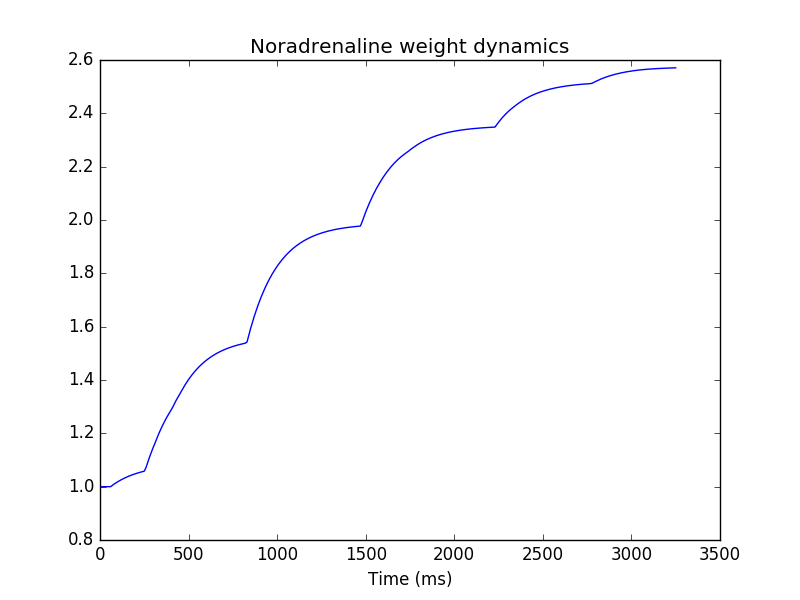
\includegraphics[width=\linewidth]{w_dynamic_250_with_nora}
	\caption{Изменение силы связи между пресинаптическим и постсинаптическим нейронами в присутствии норадреналина.}
	\label{fig:w_dynamic_250_with_nora}
\end{figure}

Второй, контрольный эксперимент без активации норадреналина показал, что без присутствия нейромедиатора сила связи между нейронами единична и не меняется на протяжении всей симуляции (рисунок ~\ref{fig:w_dynamic_250}).

\begin{figure}
	\centering
	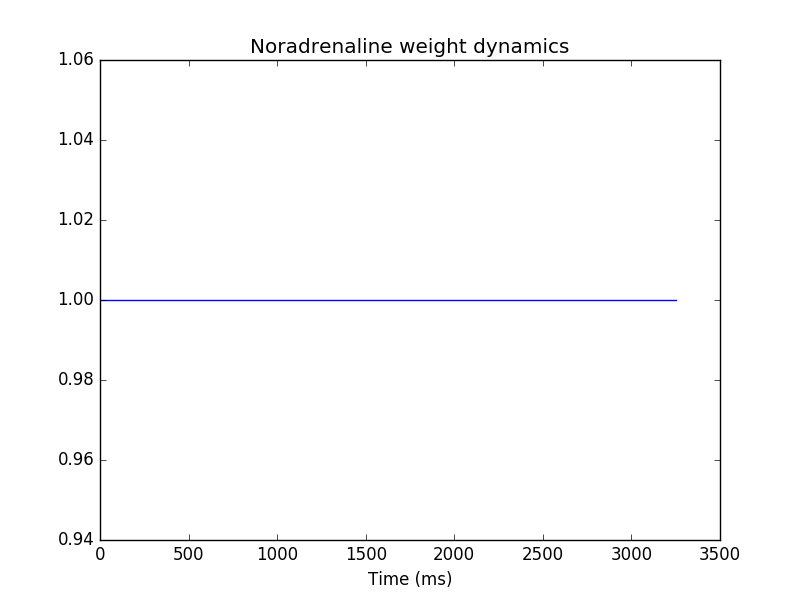
\includegraphics[width=\linewidth]{w_dynamic_250}
	\caption{Изменение силы связи между пресинаптическим и постсинаптическим нейронами в отсутствие нейромедиаторов.}
	\label{fig:w_dynamic_250}
\end{figure}